% C.26 中点四边形
\documentclass[tikz,border=4pt]{standalone}
\usepackage{ctex}
\usepackage{amsmath}
\usetikzlibrary{calc, arrows.meta}
\begin{document}
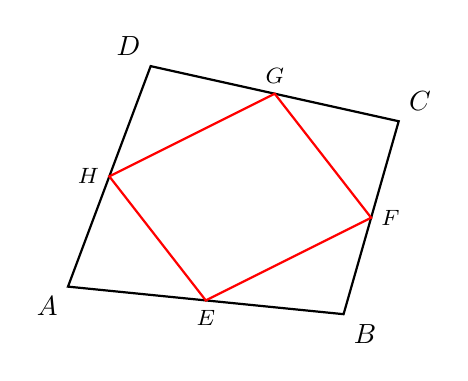
\begin{tikzpicture}[scale=0.7, thick]
  \coordinate (A) at (0,0);
  \coordinate (B) at (5,-0.5);
  \coordinate (C) at (6,3);
  \coordinate (D) at (1.5,4);
  \coordinate (E) at ($(A)!0.5!(B)$);
  \coordinate (F) at ($(B)!0.5!(C)$);
  \coordinate (G) at ($(C)!0.5!(D)$);
  \coordinate (H) at ($(D)!0.5!(A)$);
  \draw (A) -- (B) -- (C) -- (D) -- cycle;
  \draw[red] (E) -- (F) -- (G) -- (H) -- cycle;
  \node[below left] at (A) {$A$};
  \node[below right] at (B) {$B$};
  \node[above right] at (C) {$C$};
  \node[above left] at (D) {$D$};
  \node[font=\footnotesize, below] at (E) {$E$};
  \node[font=\footnotesize, right] at (F) {$F$};
  \node[font=\footnotesize, above] at (G) {$G$};
  \node[font=\footnotesize, left] at (H) {$H$};
\end{tikzpicture}
\end{document}
